\documentclass[aspectratio=169]{beamer}

% Theme and color
\usetheme{Madrid}
\usecolortheme{default}

% Packages
\usepackage[utf8]{inputenc}
\usepackage{graphicx}
\usepackage{tikz}
\usepackage{amsmath}
\usepackage{amssymb}
\usepackage{booktabs}

% TikZ libraries
\usetikzlibrary{shapes.geometric, arrows, positioning}

% Title Information
\title{A Handwritten Music Recognition System Based on Visual Object Detection and Semantic Assembly}
\author{Yuguang Yao \and Hok Seng}
\date{\today}

\begin{document}

% Slide 1: Title
\frame{\titlepage}

% Slide 2: Introduction & Motivation
\begin{frame}{Introduction \& Motivation}
    \begin{block}{What is Optical Music Recognition (OMR)?}
        \begin{itemize}
            \item Computationally read music notation in documents
            \item Invert the music encoding process to recover musical semantics
            \item Goal: Enable replayability and score editing
        \end{itemize}
    \end{block}
    
    \begin{block}{Why is OMR Challenging?}
        \begin{itemize}
            \item \textbf{2D Structure}: Unlike OCR's linear text sequences
            \item \textbf{Context-Dependent}: Symbol meaning depends on spatial relationships
            \item \textbf{Size Variability}: From tiny dots to large braces
            \item \textbf{Complex Alignment}: Overlapping beams, slurs, and symbols
        \end{itemize}
    \end{block}
    
    \vspace{0.3cm}
    \textbf{Project Goal}: End-to-end pipeline from score image $\rightarrow$ MusicXML
\end{frame}

% Slide 3: System Pipeline Overview
\begin{frame}{System Pipeline Overview}
    \begin{center}
        \resizebox{0.95\textwidth}{!}{
        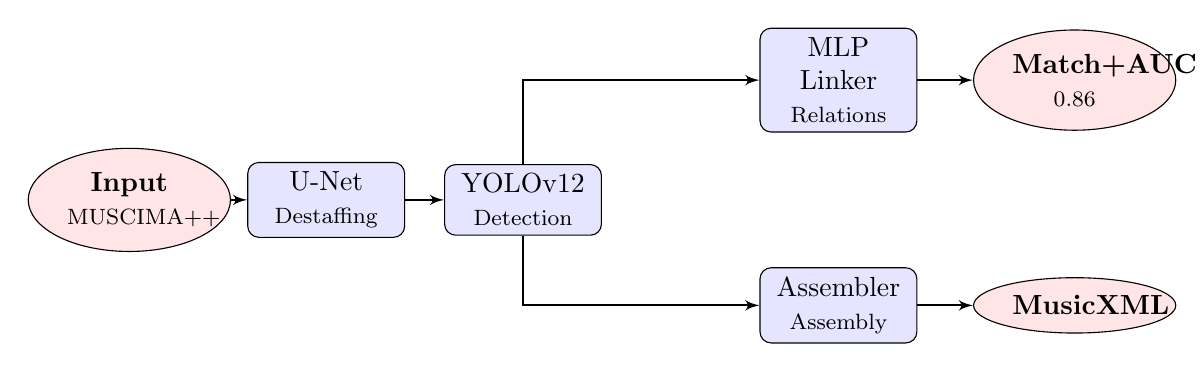
\begin{tikzpicture}[
            node distance=2.5cm, 
            auto,
            block/.style={rectangle, draw, fill=blue!10, text width=5em, text centered, rounded corners, minimum height=2.5em},
            cloud/.style={draw, ellipse, fill=red!10, minimum height=2em, text width=4.5em, text centered},
            line/.style={draw, -latex', thick}
        ]
            % Nodes
            \node [cloud] (input) {\textbf{Input}\\ \footnotesize MUSCIMA++};
            \node [block, right of=input, node distance=2.5cm] (unet) {U-Net\\ \footnotesize Destaffing};
            \node [block, right of=unet, node distance=2.5cm] (yolo) {YOLOv12\\ \footnotesize Detection};
            
            % Branching
            \node [block, above right=0.4cm and 2cm of yolo] (mlp) {MLP Linker\\ \footnotesize Relations};
            \node [block, below right=0.4cm and 2cm of yolo] (rules) {Assembler\\ \footnotesize Assembly};
            
            % End points
            \node [cloud, right of=mlp, node distance=3cm] (eval) {\textbf{Match+AUC}\\ \footnotesize 0.86};
            \node [cloud, right of=rules, node distance=3cm] (output) {\textbf{MusicXML}};
            
            % Edges
            \path [line] (input) -- (unet);
            \path [line] (unet) -- (yolo);
            \path [line] (yolo) |- (mlp);
            \path [line] (yolo) |- (rules);
            \path [line] (mlp) -- (eval);
            \path [line] (rules) -- (output);
        \end{tikzpicture}
        }
    \end{center}
    
    \vspace{0.5cm}
    \begin{block}{Four Main Modules}
        \textbf{U-Net} $\rightarrow$ \textbf{YOLO} $\rightarrow$ \textbf{MLP} $\rightarrow$ \textbf{Assembler}
    \end{block}
\end{frame}

% Slide 4: Module 1 - U-Net Preprocessing
\begin{frame}{Module 1: Data Preprocessing (U-Net)}
    \begin{columns}
        \begin{column}{0.5\textwidth}
            \begin{block}{U-Net Architecture}
                \begin{itemize}
                    \item Encoder-decoder with skip connections
                    \item Pixel-wise classification
                    \item Separates symbols from staff lines
                \end{itemize}
            \end{block}
            
            \begin{block}{Preprocessing Pipeline}
                \begin{enumerate}
                    \item \textbf{Staff Removal}: Destaff to improve SNR
                    \item \textbf{Image Cropping}: $640 \times 640$ patches
                    \item \textbf{Annotation Conversion}: XML $\rightarrow$ YOLO format
                \end{enumerate}
            \end{block}
        \end{column}
        
        \begin{column}{0.5\textwidth}
            \begin{figure}
                \centering
                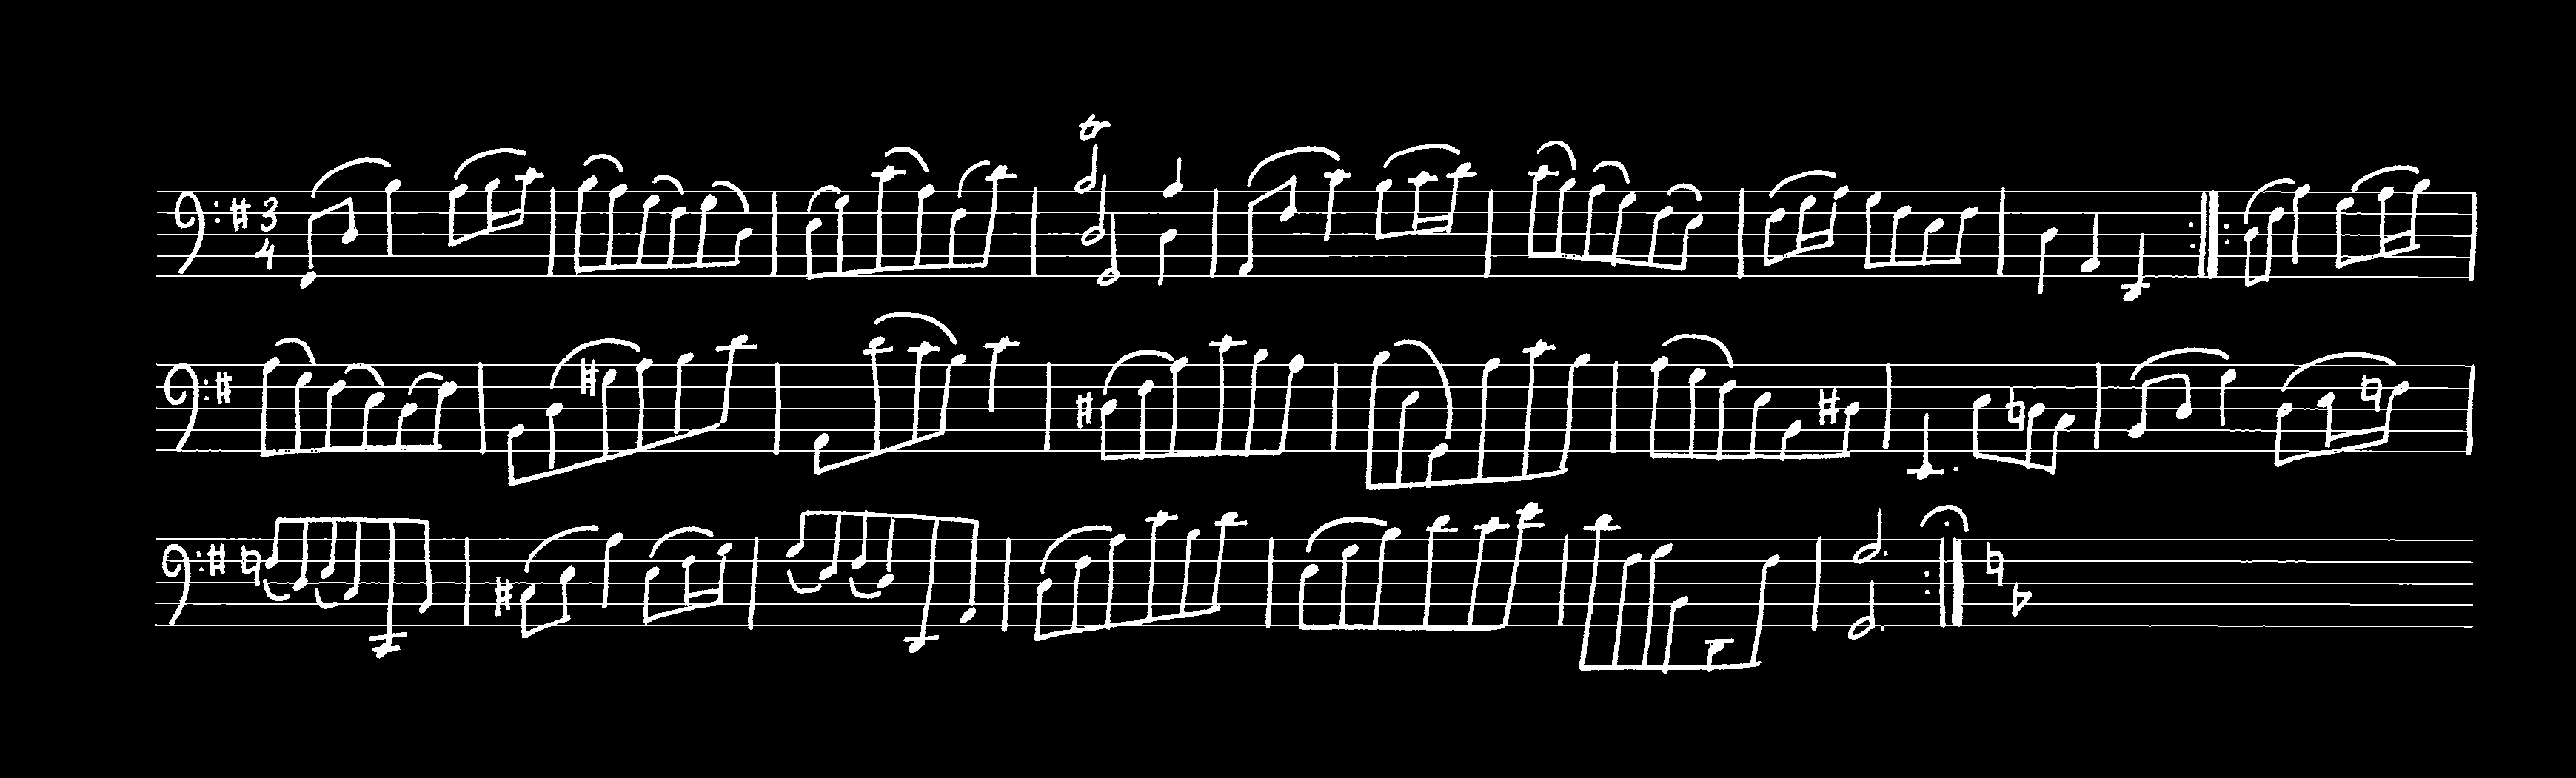
\includegraphics[width=\textwidth]{p009_reproduced/p009.png}
                \caption{Original input}
            \end{figure}
            
            \begin{figure}
                \centering
                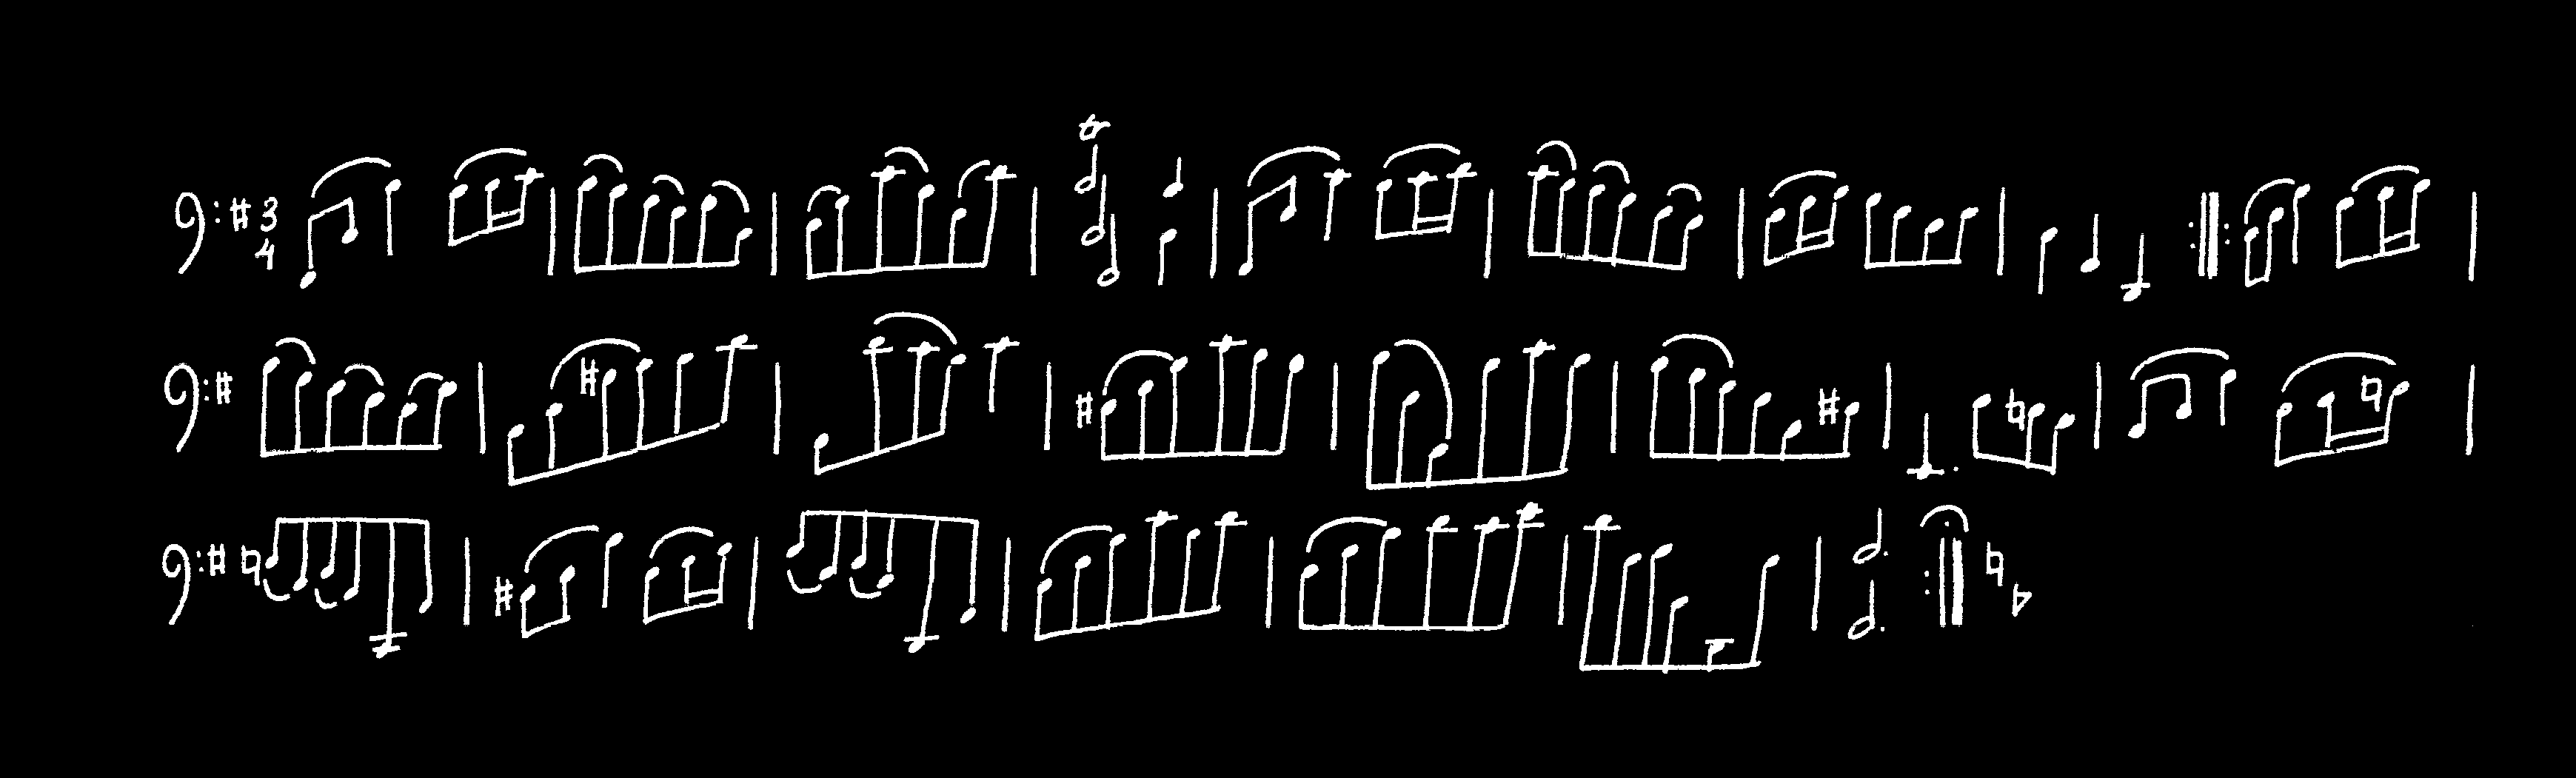
\includegraphics[width=\textwidth]{p009_reproduced/03_unet_cleaned.png}
                \caption{After U-Net destaffing}
            \end{figure}
        \end{column}
    \end{columns}
\end{frame}

% Slide 5: Module 2 - YOLO Detection
\begin{frame}{Module 2: Visual Detection (YOLOv12)}
    \begin{columns}
        \begin{column}{0.6\textwidth}
            \begin{block}{YOLO Configuration}
                \begin{itemize}
                    \item \textbf{Model}: YOLOv12-Large
                    \item \textbf{Classes}: 117 symbol types
                    \item \textbf{Training}: 100 epochs, SGD optimizer
                    \item \textbf{Input Size}: $640 \times 640$ pixels
                    \item \textbf{Augmentation}: Mosaic for robustness
                \end{itemize}
            \end{block}
            
            \begin{block}{Symbol Categories}
                Noteheads, Stems, Beams, Flags, Rests, Accidentals, Clefs, Time Signatures, Barlines, Tuplet Brackets, etc.
            \end{block}
            
            \begin{block}{Performance}
                High mAP on common symbols $\rightarrow$ Solid foundation for assembly
            \end{block}
        \end{column}
        
        \begin{column}{0.4\textwidth}
            \begin{figure}
                \centering
                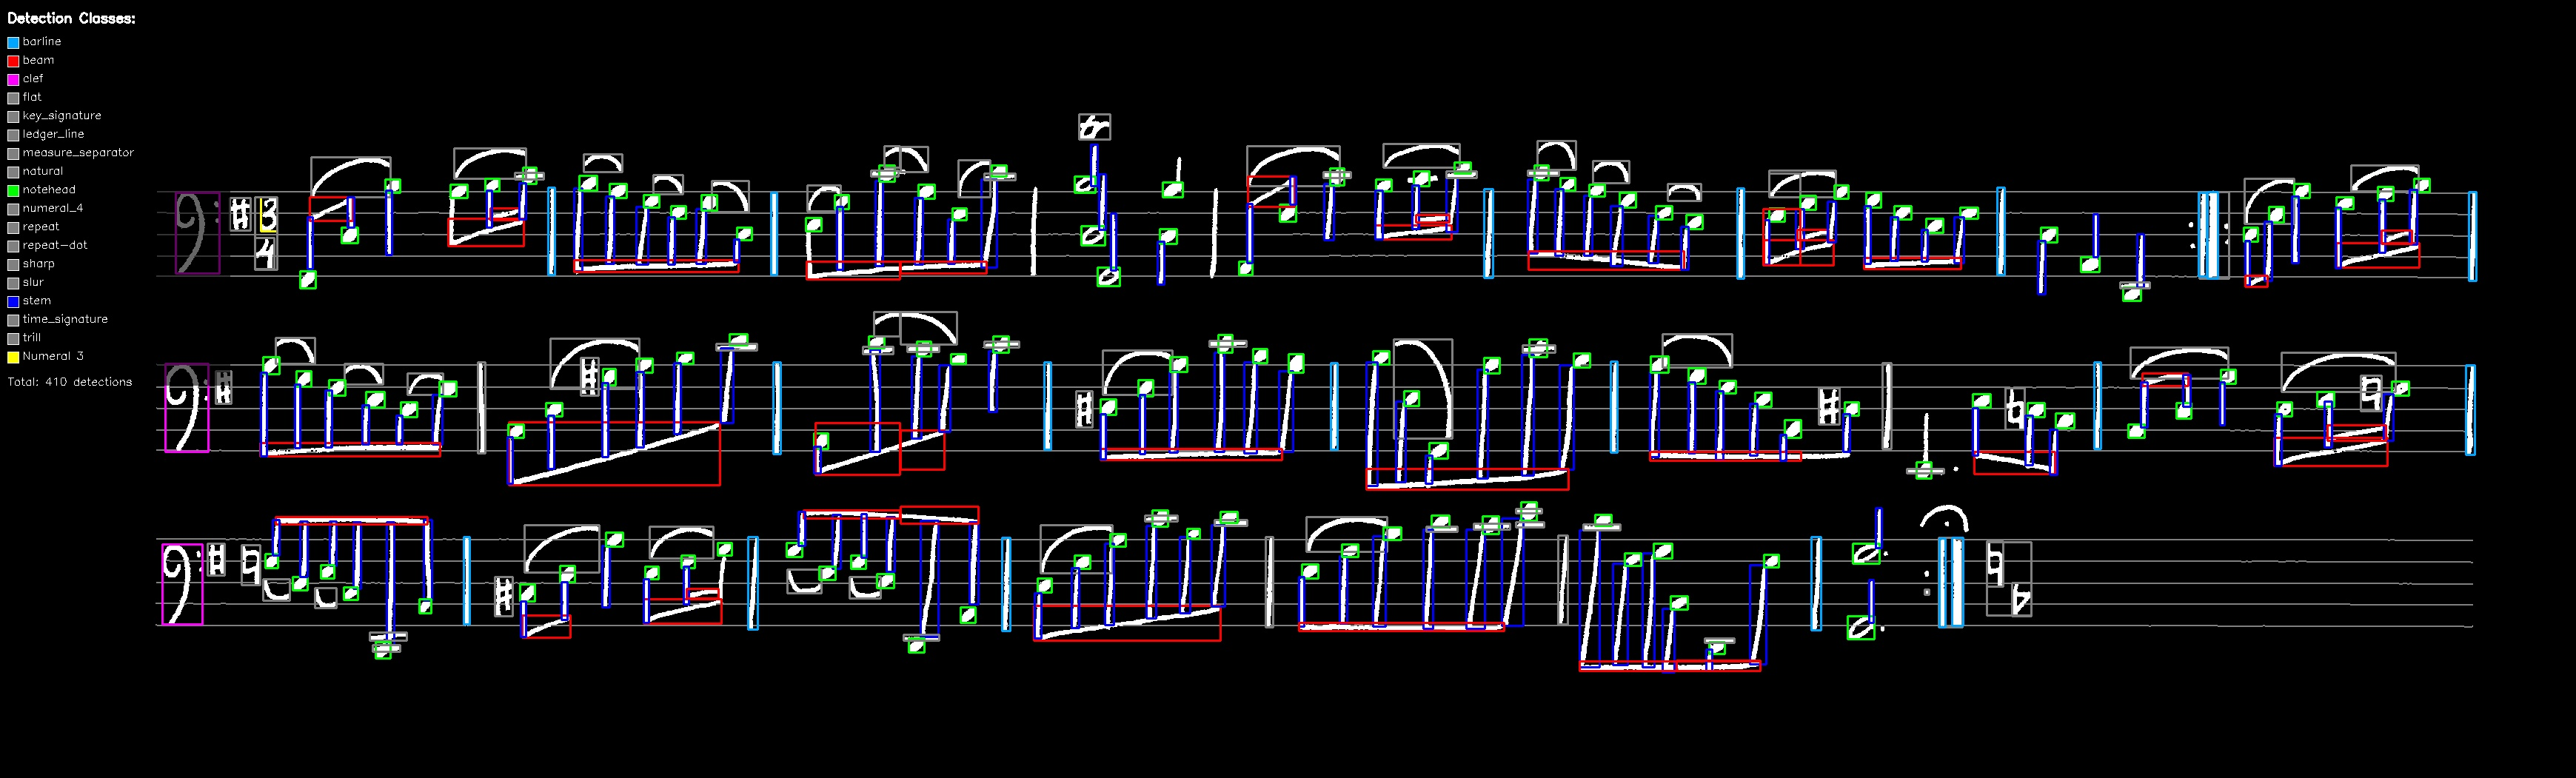
\includegraphics[width=\textwidth]{p009_reproduced/04_yolo_detections.jpg}
                \caption{YOLOv12 detection results}
            \end{figure}
        \end{column}
    \end{columns}
\end{frame}

% Slide 6: Module 3 - MLP Linker
\begin{frame}{Module 3: Relation Prediction (MLP Linker)}
    \begin{block}{Problem Formulation}
        Link prediction on fully connected graph: each detected symbol = node
    \end{block}
    
    \begin{columns}
        \begin{column}{0.5\textwidth}
            \begin{block}{Feature Engineering}
                \textbf{Geometric Features}:
                \begin{itemize}
                    \item Relative distance: $d_x, d_y$
                    \item Normalized bbox coordinates
                    \item IoU overlap ratio
                \end{itemize}
                
                \vspace{0.3cm}
                \textbf{Semantic Features}:
                \begin{itemize}
                    \item Class embeddings: $\mathbf{e}_u, \mathbf{e}_v \in \mathbb{R}^{32}$
                    \item Concatenated: $[\mathbf{e}_u; \mathbf{e}_v] \in \mathbb{R}^{64}$
                    \item Captures class-specific patterns
                \end{itemize}
            \end{block}
        \end{column}
        
        \begin{column}{0.5\textwidth}
            \begin{block}{MLP Architecture}
                \begin{itemize}
                    \item 3 hidden layers with ReLU
                    \item Output: $P(u \to v) \in [0, 1]$
                    \item Constructs \textbf{Notation Graph}
                \end{itemize}
            \end{block}
            
            \begin{figure}
                \centering
                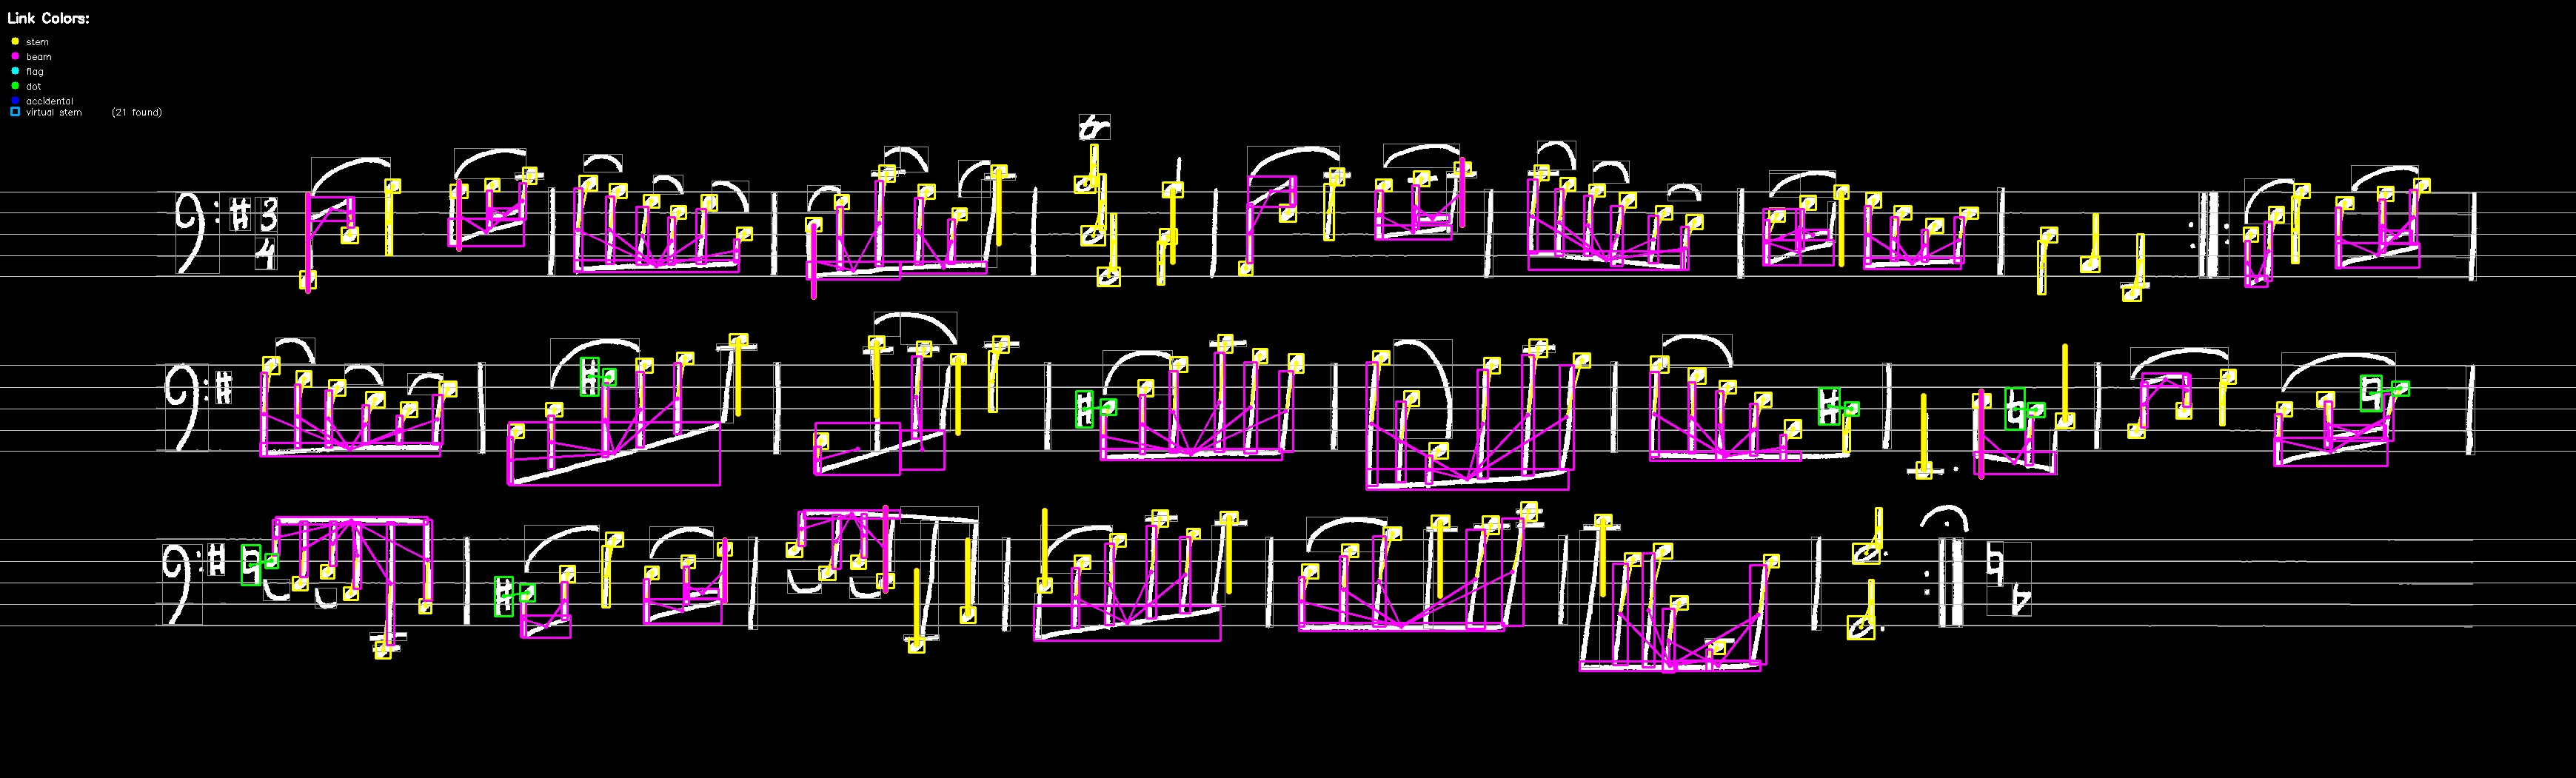
\includegraphics[width=0.9\textwidth]{p009_reproduced/05_assembled_links.jpg}
                \caption{Notation graph with relationships}
            \end{figure}
        \end{column}
    \end{columns}
\end{frame}

% Slide 7: MLP Evaluation & Results
\begin{frame}{MLP Evaluation \& Results}
    \begin{block}{Match+AUC Metric}
        Combines two complementary aspects:
        \begin{itemize}
            \item \textbf{Match Score}: Precision of predicted edges vs. ground truth
            \item \textbf{AUC}: Ranking quality of edge probabilities
        \end{itemize}
    \end{block}
    
    \begin{center}
        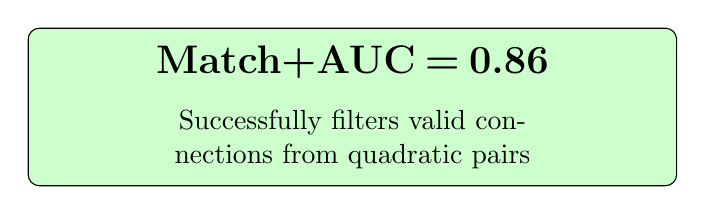
\begin{tikzpicture}
            \node[draw, fill=green!20, rounded corners, text width=8cm, text centered, minimum height=2cm] {
                \Large \textbf{Match+AUC = 0.86}\\
                \vspace{0.3cm}
                \normalsize Successfully filters valid connections from quadratic pairs
            };
        \end{tikzpicture}
    \end{center}
    
    \vspace{0.5cm}
    \begin{block}{Key Achievement}
        MLP effectively learns geometric and semantic patterns of symbol relationships, enabling robust notation graph construction.
    \end{block}
\end{frame}

% Slide 8: Module 4 - Semantic Assembly
\begin{frame}{Module 4: Semantic Assembly}
    \begin{block}{Six-Phase Rule-Based Assembly Pipeline}
        \begin{enumerate}
            \item \textbf{System \& Staff Grouping}: Organize staves into musical rows
            \item \textbf{Measure Slicing}: Horizontal segmentation via barline detection
            \item \textbf{Symbol Assembly}: Link noteheads $\rightarrow$ stems $\rightarrow$ beams $\rightarrow$ dots
            \item \textbf{Attribute Recognition}: Detect clef, key signature, time signature
            \item \textbf{Tuplet Detection}: Cascaded rules (Bracket $\rightarrow$ Beam $\rightarrow$ Numeral)
            \item \textbf{Pitch Determination}: Convert geometric positions to musical pitches
        \end{enumerate}
    \end{block}
    
    \begin{columns}
        \begin{column}{0.5\textwidth}
            \begin{figure}
                \centering
                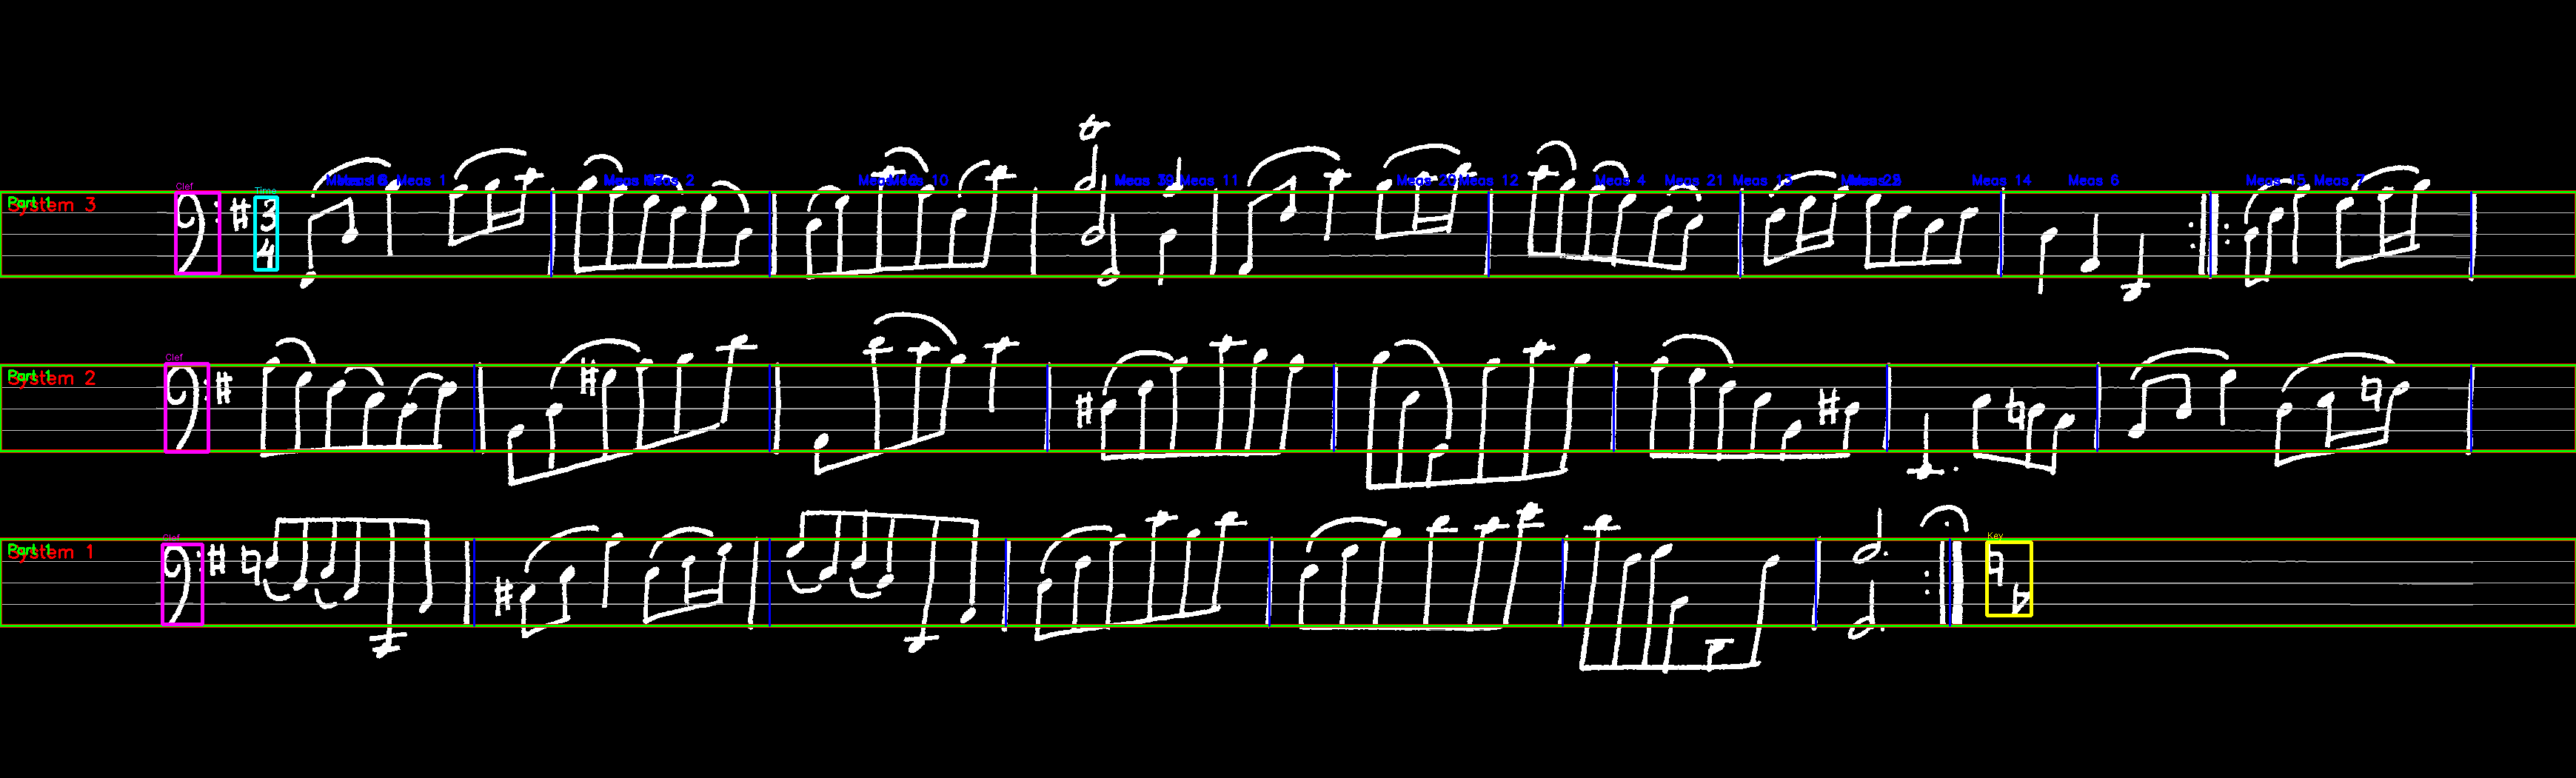
\includegraphics[width=0.9\textwidth]{p009_reproduced/06_system_structure.png}
                \caption{System structure}
            \end{figure}
        \end{column}
        
        \begin{column}{0.5\textwidth}
            \begin{block}{Key Features}
                \begin{itemize}
                    \item State persistence for attributes
                    \item Virtual stem creation
                    \item Priority-based rule ordering
                \end{itemize}
            \end{block}
        \end{column}
    \end{columns}
\end{frame}

% Slide 9: Key Technical Challenge - Tuplet Detection
\begin{frame}{Technical Challenge: Tuplet Detection}
    \begin{block}{Cascaded Rule Set (Decreasing Constraint Strength)}
        \begin{enumerate}
            \item \textbf{Rule 1 - Bracket-Based} [Highest Priority]
            \begin{itemize}
                \item Search for \texttt{tuple\_bracket} covering exactly 3 notes
                \item Relaxed: accepts without \texttt{numeral\_3} if 3 notes present
            \end{itemize}
            
            \item \textbf{Rule 2 - Beam-Based} [Second Priority]
            \begin{itemize}
                \item Beams linking 3k stems with nearby \texttt{numeral\_3}
                \item \textbf{Exclusion}: Finger numbers (vertically aligned above single note)
            \end{itemize}
            
            \item \textbf{Rule 3 - Numeral-Centered} [Lower Priority]
            \begin{itemize}
                \item Find 3 closest notes to isolated \texttt{numeral\_3}
                \item Exclude time signature numerals
            \end{itemize}
            
            \item \textbf{Rule 4 - Duration Modification}
            \begin{itemize}
                \item Apply: $duration_{xml} = base\_duration \times \frac{2}{3}$
            \end{itemize}
            
            \item \textbf{Rule 5 - Sanity Check} [Fallback]
            \begin{itemize}
                \item Detect measure overflow, search for 3 identical-duration notes
            \end{itemize}
        \end{enumerate}
    \end{block}
\end{frame}

% Slide 10: Results & MusicXML Output
\begin{frame}{Results \& MusicXML Output}
    \begin{columns}
        \begin{column}{0.5\textwidth}
            \begin{block}{Achievements}
                \begin{itemize}
                    \item \textbf{End-to-End}: Image $\rightarrow$ MusicXML
                    \item \textbf{Compatible}: Opens in MuseScore
                    \item \textbf{Polyphonic}: Handles multiple voices
                    \item \textbf{Complex Rhythms}: Tuplets, dotted notes
                \end{itemize}
            \end{block}
            
            \begin{block}{Future Improvements}
                \begin{enumerate}
                    \item \textbf{Enhanced Linker}: Small models for sub-processes
                    \item \textbf{More Symbol Types}: Expand coverage
                    \item \textbf{Interactive Processing}: User-modifiable probabilities
                \end{enumerate}
            \end{block}
        \end{column}
        
        \begin{column}{0.5\textwidth}
            \begin{figure}
                \centering
                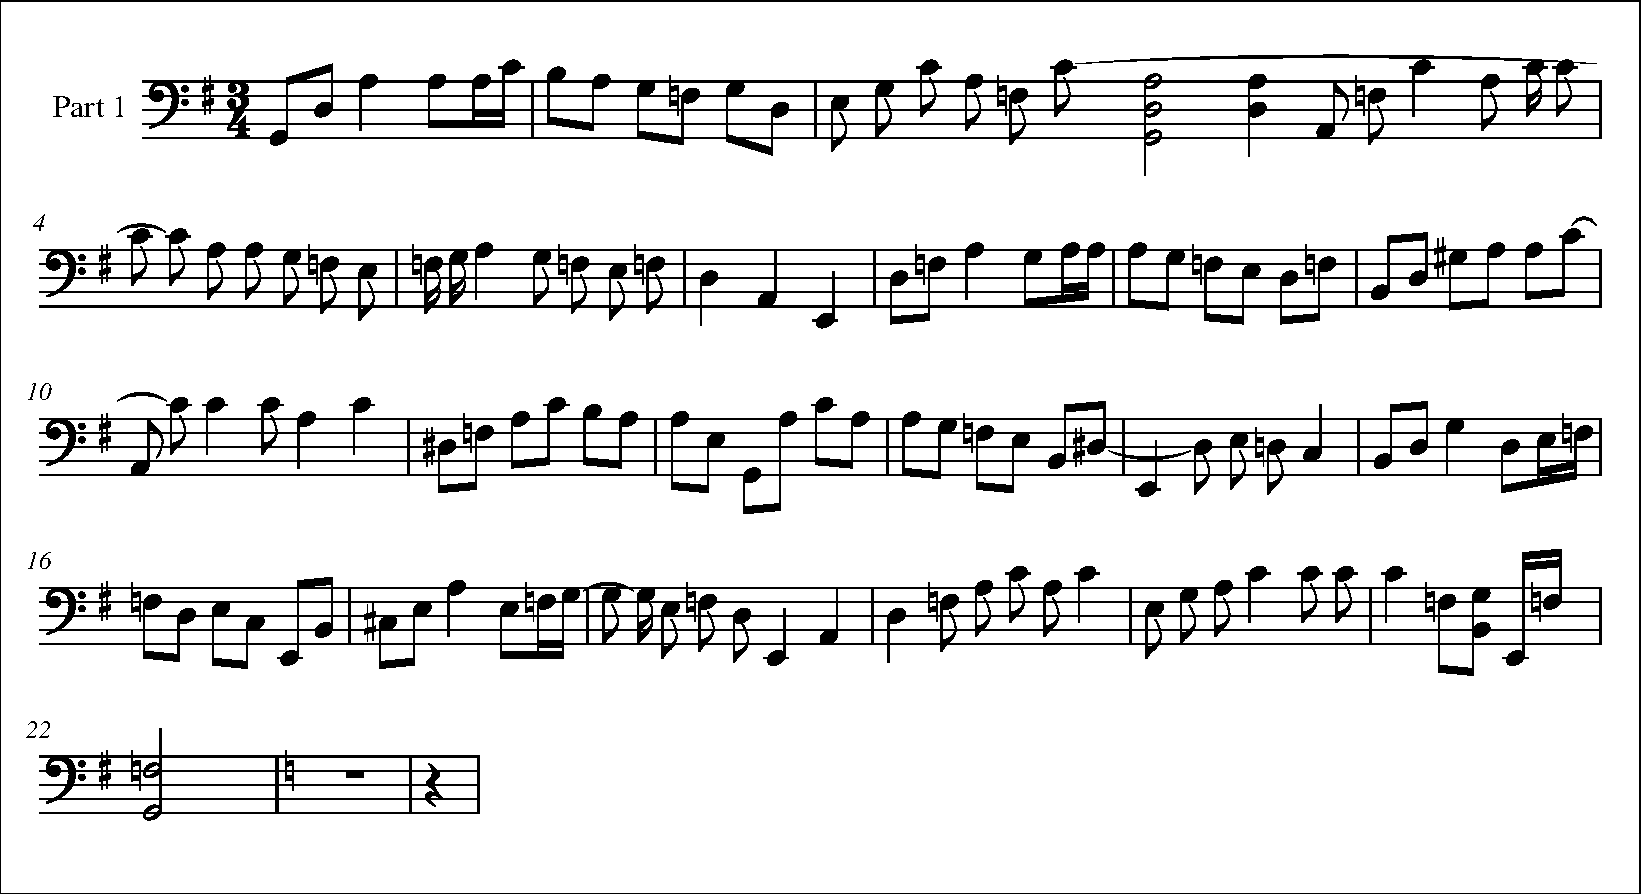
\includegraphics[width=0.95\textwidth]{p009_reproduced/output.pdf}
                \caption{Final MusicXML output rendered as musical notation}
            \end{figure}
            
            \vspace{0.3cm}
            \begin{center}
                \Large \textbf{Thank You!}\\
                \vspace{0.2cm}
                \normalsize Questions?
            \end{center}
        \end{column}
    \end{columns}
\end{frame}

\end{document}
